
%% ==================================================================
%% DOCUMENT CLASS ---------------------------------------------------
%% ==================================================================

%%    Uncomment the following for <article> mode

\documentclass[pdf,oneside]{book}

%% ==================================================================
%% PREAMBLE ---------------------------------------------------------
%% ==================================================================

\usepackage{type1cm}
\usepackage{fullpage}
%
\usepackage{myoxygen}
\usepackage[sort]{natbib}
%\usepackage{apaish}
\usepackage{color,atbeginend}
\usepackage{fancyhdr,verbatim,extramarks}
\usepackage{listings,arydshln,hhline,graphicx}
\usepackage{helvet}
\usepackage{courier}
%\usepackage{lastpage}
\usepackage[small,compact]{titlesec}
\usepackage[english]{babel}
\usepackage{hyperref}
\usepackage{listings}
\usepackage{pdfpages}
\usepackage[titletoc]{appendix}
%\usepackage[T1]{fontenc}
%\usepackage[latin9]{inputenc}
\usepackage{lmodern} % Use the modern font family; this renders T1
                     % fonts, which do not show up as being "blurry" in
                     % Adobe Acrobat
\usepackage{float}
\usepackage{amsmath}
\usepackage{graphicx}
\usepackage{babel}
\usepackage{enumitem}
\usepackage{tabularx}

\floatname{example}{Example}

\newcommand{\indexsolver}[1]{\index{#1 solver}\index{solver!#1}}

\newcommand{\code}[1]{\textmd{\texttt{#1}}}
\newcommand{\todo}[1]{\textbf{\textit{TODO: #1}}}
%\newcommand{\comment}[1]{\marginpar{\textit{#1}}}
\newcommand{\st}{\textrm{s.t.}}

\newenvironment{notebox}%
  {\begin{table}\begin{center}\begin{Sbox}\begin{minipage}{.8\textwidth}{\bf NOTE:}}
  {\end{minipage}\end{Sbox}\fbox{\TheSbox}\end{center}\end{table}}

\newenvironment{Xnotebox}%
  {\begin{table}\begin{center}\begin{svgraybox}\begin{minipage}{.8\textwidth}{\bf NOTE:}}
  {\end{minipage}\end{svgraybox}\end{center}\end{table}}

\lstnewenvironment{unknownListing}%
  {\lstset{
    keepspaces=true,
    aboveskip=0.3em,
    belowskip=0.3em,
    xleftmargin=1.5em,
    xrightmargin=1.5em,
    showspaces=false,
    showstringspaces=false,
    columns=fullflexible,
    frame=single,
    basicstyle=\footnotesize\ttfamily ,
    backgroundcolor=\color{white},
	escapechar=`
    }}
  {}

\lstnewenvironment{qlist}%
  {\lstset{
    keepspaces=true,
    aboveskip=0.3em,
    belowskip=0.3em,
    xleftmargin=1.5em,
    xrightmargin=1.5em,
    showspaces=false,
    showstringspaces=false,
    columns=fullflexible,
    frame=single,
    basicstyle=\footnotesize\ttfamily ,
    backgroundcolor=\color{white},
    language=Python
    }}
  {}

\lstnewenvironment{qautobreaklist}%
  {\lstset{
    keepspaces=true,
    aboveskip=0.3em,
    belowskip=0.3em,
    xleftmargin=1.5em,
    xrightmargin=1.5em,
    showspaces=false,
    showstringspaces=false,
    columns=fullflexible,
    frame=single,
    breaklines=true,
    breakatwhitespace=true,
    prebreak={\textbackslash},
    basicstyle=\footnotesize\ttfamily ,
    backgroundcolor=\color{white},
    language=Python
    }}
  {}


%
% Syntax: \listing{<filename>}{<anchor>}{<firstline>}{<lastline>}
%
% NOTE: the firstline and lastline data is automatically generated.  For example:
%
%   \listing{foo}{bar}
%
% is initialized to find the 'bar' anchor in file 'foo'.  Additionally, if we have
%
%   \listing{foo}{}
%
% then the entire file 'foo' is include.
%
\newcommand{\listing}[4]{\lstinputlisting[firstline=#3,lastline=#4,
    keepspaces=true,
    aboveskip=0.3em,
    belowskip=0.3em,
    xleftmargin=1.5em,
    xrightmargin=1.5em,
    showspaces=false,
    showstringspaces=false,
    columns=fullflexible,
    frame=single,
    basicstyle=\footnotesize\ttfamily ,
    backgroundcolor=\color{white},
    language=Python
    ]{#1}}

\newcommand{\unknownInputListing}[4]{\lstinputlisting[firstline=#3,lastline=#4,
    keepspaces=true,
    aboveskip=0.3em,
    belowskip=0.3em,
    xleftmargin=1.5em,
    xrightmargin=1.5em,
    showspaces=false,
    showstringspaces=false,
    columns=fullflexible,
    breaklines=true,
    breakatwhitespace=true,
    frame=single,
    basicstyle=\footnotesize\ttfamily ,
    backgroundcolor=\color{white},
    ]{#1}}

\newcommand{\unknownInputListingFixed}[4]{\lstinputlisting[firstline=#3,lastline=#4,
    keepspaces=true,
    aboveskip=0.3em,
    belowskip=0.3em,
    xleftmargin=1.5em,
    xrightmargin=1.5em,
    showspaces=false,
    showstringspaces=false,
    columns=fullflexible,
    breaklines=true,
    breakatwhitespace=true,
    frame=single,
    basicstyle=\footnotesize\ttfamily ,
    backgroundcolor=\color{white},
    ]{#1}}

\newcommand{\autobreaklisting}[4]{\lstinputlisting[firstline=#3,lastline=#4,
    keepspaces=true,
    aboveskip=0.3em,
    belowskip=0.3em,
    xleftmargin=1.5em,
    xrightmargin=1.5em,
    showspaces=false,
    showstringspaces=false,
    columns=fullflexible,
    frame=single,
    breaklines=true,
    breakatwhitespace=true,
    prebreak={\textbackslash},
    basicstyle=\footnotesize\ttfamily ,
    backgroundcolor=\color{white},
    language=Python
    ]{#1}}


\newcommand{\scriptsizelisting}[4]{\lstinputlisting[firstline=#3,lastline=#4,
    keepspaces=true,
    aboveskip=0.3em,
    belowskip=0.3em,
    xleftmargin=1.5em,
    xrightmargin=1.5em,
    showspaces=false,
    showstringspaces=false,
    columns=fullflexible,
    frame=single,
    basicstyle=\scriptsize\ttfamily ,
    backgroundcolor=\color{white},
    language=Python
    ]{#1}}

\newcommand{\tinylisting}[4]{\lstinputlisting[firstline=#3,lastline=#4,
    keepspaces=true,
    aboveskip=0.3em,
    belowskip=0.3em,
    xleftmargin=1.5em,
    xrightmargin=1.5em,
    showspaces=false,
    showstringspaces=false,
    columns=fullflexible,
    frame=single,
    basicstyle=\tiny\ttfamily ,
    backgroundcolor=\color{white},
    language=Python
    ]{#1}}


\newcommand\docTitle{Installation Guide}

% ---------------------------------------------------------------- %
%
% Set the title, author, and date
  \title{\sc Water Security Toolkit \docTitle:\\Version 1.0}

  \author{\\Editors:\\
\\
Terranna Haxton\\
Center for Environmental Solutions and Emergency Response\\
Office of Research and Development\\
U.S. Environmental Protection Agency\\\
Cincinnati, OH 45256\\
\\
Katherine A. Klise\\
Geoscience Research and Applications Group\\
Sandia National Laboratories \\
PO Box 5800 MS 0751 \\
Albuquerque, NM 87185 \\
\\
  }
  
  \date{}

%\SANDprintDate{Jan 2013}
%\author{J. Berry, E. Boman, L.A. Riesen, W.E. Hart, C.A. Phillips, J.-P. Watson}

\hypersetup{colorlinks=false}
\parindent 0mm
\parskip = 2mm
%\AfterBegin{itemize}{\setlength{\itemsep}{1.75mm}}
%\AfterBegin{enumerate}{\setlength{\itemsep}{1.75mm}}
%\AfterBegin{description}{\setlength{\itemsep}{1.75mm}}
%\titleformat{\chapter}[hang]{\bf\large}{\thechapter\quad}{2mm}{\large}[]
%\titlespacing{\chapter}{0pt}{0mm}{5mm}

%% Set up the XML language
%\lstdefinestyle{XML}{language=XML, basicstyle={\ttfamily},
  %usekeywordsintag=true, alsoletter={-}, escapechar={\#},
  %markfirstintag=true, morestring=[b]{''}, mathescape=true,
  %keywordstyle=\sffamily\bfseries, stringstyle=\rmfamily\textsl }
%%% End of preamble --------------------------------------------------

\lstset{aboveskip=1em,belowskip=1em,showspaces=false,showstringspaces=false}
\lstset{frame=single,
  basicstyle=\footnotesize ,
  backgroundcolor=\color{white}}

\newlength{\topheight}
\setlength{\topheight}{1.0in}

%% ==================================================================
%% MAIN DOCUMENT ----------------------------------------------------
%% ==================================================================

\begin{document}
  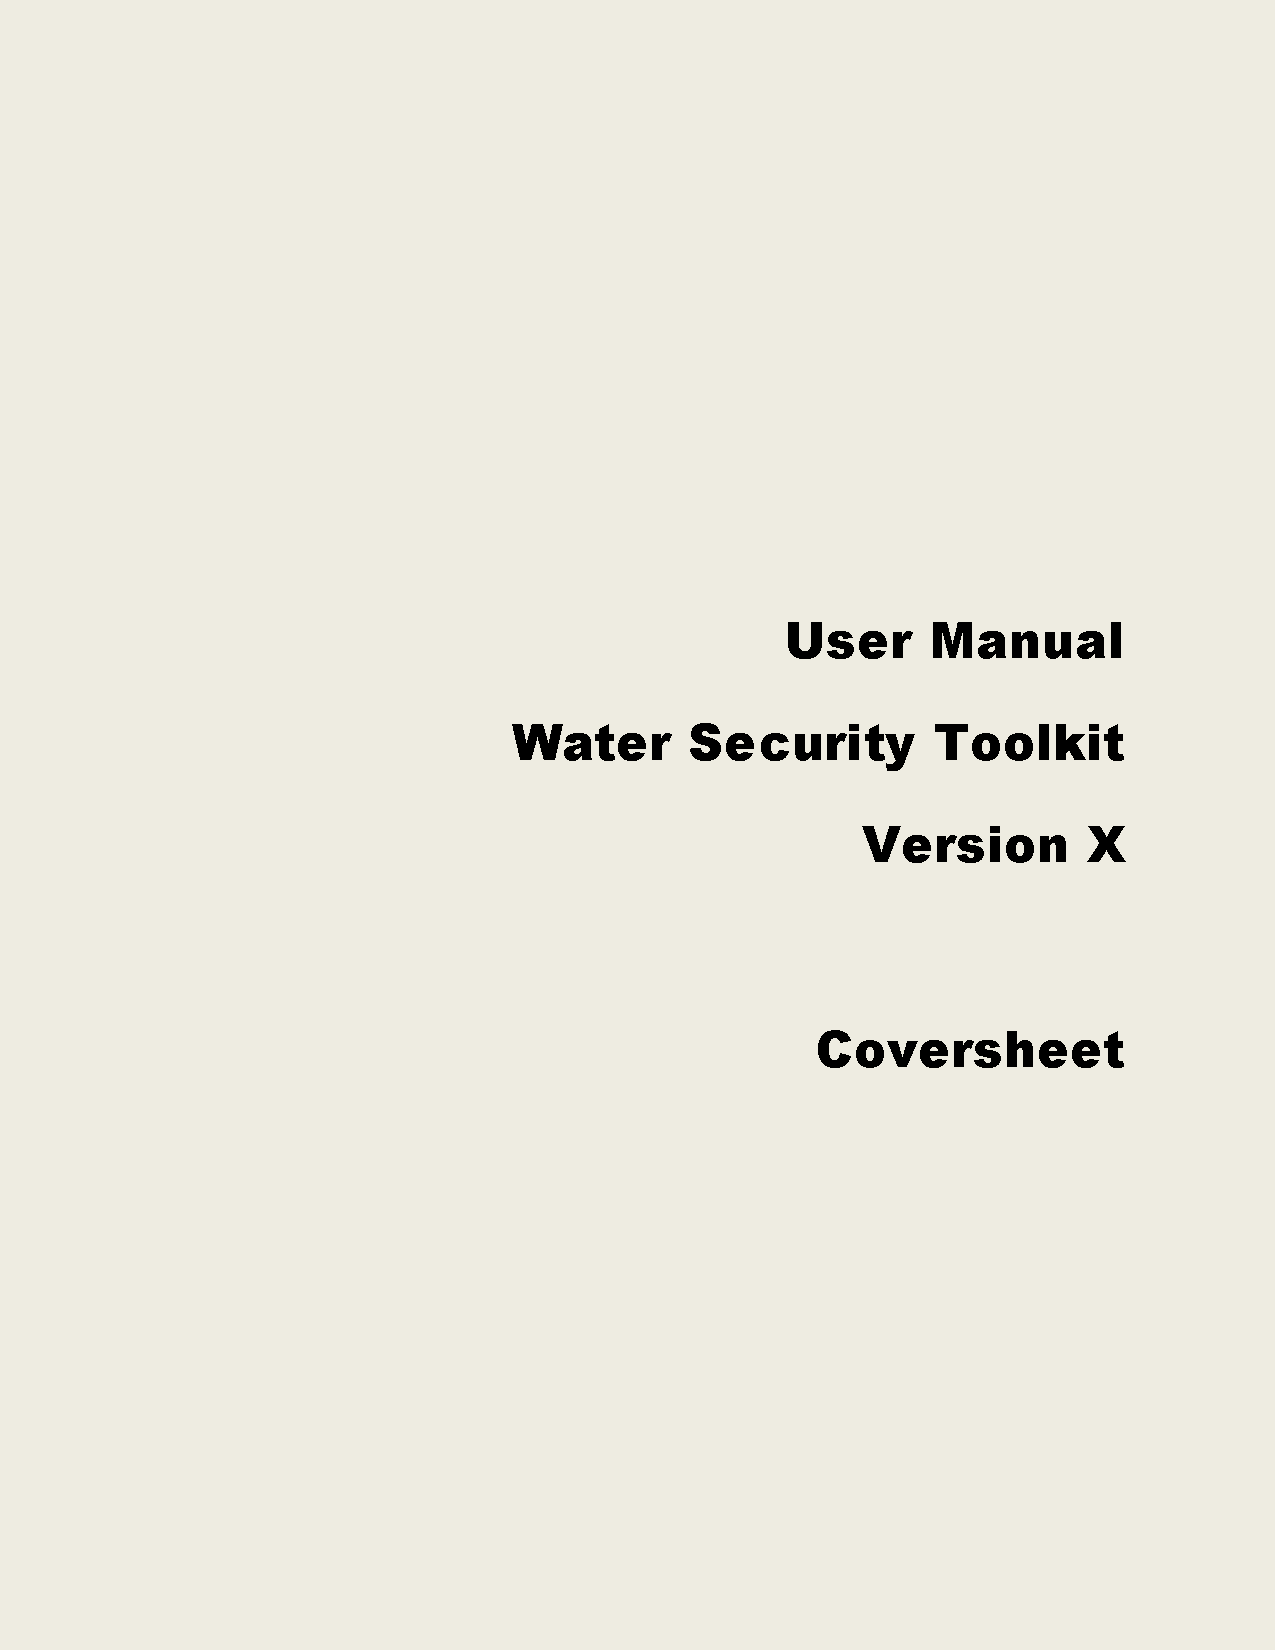
\includepdf[pages={1}]{coversheet_blank.pdf}
  \maketitle

  \pagenumbering{roman}
  \clearpage
  The U.S. Environmental Protection Agency (EPA) through its Office of 
Research and Development funded and collaborated in the research described 
here under an Interagency Agreement (IA \# DW8992192801 and \# DW8992450201) with the Department 
of Energy's Sandia National Laboratories. It has been subject to the Agency's 
review and has been approved for publication. Note that approval does not 
signify that the contents necessarily reflect the views of the Agency. 
Mention of trade names, products, or services does not convey official 
EPA approval, endorsement, or recommendation.

\bigskip
\bigskip

{\fontseries{b}\selectfont NOTICE:} 
This report was prepared as an account of work sponsored
by an agency of the United States Government. Accordingly, the United
States Government retains a nonexclusive, royalty-free license to
publish or reproduce the published form of this contribution, or allow
others to do so for United States Government purposes. Neither Sandia
Corporation, the United States Government, nor any agency thereof, nor
any of their employees makes any warranty, express or implied, or
assumes any legal liability or responsibility for the accuracy,
completeness, or usefulness of any information, apparatus, product, or
process disclosed, or represents that its use would not infringe
privately-owned rights. Reference herein to any specific commercial
product, process, or service by trade name, trademark, manufacturer,
or otherwise does not necessarily constitute or imply its endorsement,
recommendation, or favoring by Sandia Corporation, the United States
Government, or any agency thereof. The views and opinions expressed
herein do not necessarily state or reflect those of Sandia
Corporation, the United States Government or any agency thereof.

\bigskip
\bigskip

Questions concerning this document or its application should be
addressed to:

\makebox[3.4in][t]{
\begin{minipage}[c][\topheight][t]{3.4in}
Terra Haxton \\
Center for Environmental Solutions and Emergency Response\\
Office of Research and Development\\
U.S. Environmental Protection Agency\\
Cincinnati, OH 45268\\
Haxton.Terra@epamail.epa.gov\\
513-569-7810\\
\end{minipage}
}
\makebox[3.5in][c]{
\begin{minipage}[c][\topheight][t]{3.0in}
\begin{center}

\includegraphics[width=1.2in]{graphics/EPAbwlogo}
\end{center}
\end{minipage}
}

  
  %\clearpage
  %\chapter*{Forward}
  %In July of 1970, the White House and Congress worked together to establish 
the United States Environmental Protection Agency (EPA) in response to the 
growing public demand for cleaner water, air, and land. The Agency was assigned 
the daunting task of repairing the damage already done to the natural 
environment and establishing new criteria to guide Americans in making a cleaner 
environment a reality. Since 1970, EPA has worked with federal, state, tribal, 
and local partners to advance its mission to protect human health and the 
environment.

EPA leads the nation's environmental science, research, education, and assessment 
efforts. With more than 17,000 employees across the country, EPA works to 
research, develop, and enforce regulations that implement environmental laws 
enacted by Congress. In recent years, between 40 and 50 percent of EPA's 
enacted budgets have provided direct support through grants to State 
environmental programs. At laboratories located throughout the nation, the 
Agency works to assess environmental conditions and to identify, understand, and 
solve current and future environmental problems. The Agency works through its 
headquarters and regional offices with over 10,000 industries, businesses, 
nonprofit organizations, and state and local governments, on over 40 
voluntary pollution prevention programs and energy conservation efforts. 

Under existing laws and recent Homeland Security Presidential Directives, EPA 
has been called upon to play a vital role in helping to secure the nation 
against foreign and domestic enemies. The National Homeland Security Research 
Center (NHSRC) was formed in 2002 to conduct research in support of EPA's role 
in homeland security. NHSRC research efforts focus on five areas: water 
infrastructure protection, threat and consequence assessment, decontamination 
and consequence management, response capability enhancement, and homeland 
security technology testing and evaluation. EPA is the lead federal agency 
for drinking water and waste water systems and NHSRC is working to reduce 
system vulnerabilities, prevent and prepare for terrorist attacks, minimize 
public health impacts and infrastructure damage, and enhance recovery efforts. 

This \docTitle\ for the Water Security Toolkit software package is published 
and made available by EPA's Office of Research and Development to assist the 
water community in improving the security of our nation's drinking water.

\vspace*{\baselineskip}
\vspace*{\baselineskip}

\begin{tabular}{ll}
 & Gregory Sayles, Ph.D., Acting Director \\

& National Homeland Security Research Center \\
& Office of Research and Development \\
& U. S. Environmental Protection Agency
\end{tabular}


  \clearpage
  \chapter*{License Notice}
  The Water Security Toolkit (WST) v.\wstversion

Copyright \copyright\ 2012-2019 Sandia Corporation. Under the terms of Contract
DE-AC04-94AL85000, there is a non-exclusive license for use of this work
by or on behalf of the U.S. government. 

This software is distributed under the Revised BSD License (see below).  In
addition, WST leverages a variety of third-party software packages, which
have separate licensing policies:

\begin{tabularx}{\textwidth}{p{0.5in}lX}
&\bf Acro & Revised BSD License \\
&\bf argparse & Python Software Foundation License \\
&\bf Boost & Boost Software License \\
&\bf Coopr & Revised BSD License \\
&\bf Coverage & BSD License \\
&\bf Distribute & Python Software Foundation License /  Zope Public License \\
&\bf EPANET 2.00.12 & Public Domain \\
&\bf EPANET-ERD & Revised BSD License \\
&\bf EPANET-MSX & GNU Lesser General Public License (LGPL) v.3 \\
&\bf gcovr & Revised BSD License \\
&\bf GRASP & AT\&T Commercial License for noncommercial use; includes
  \code{randomsample} and \code{sideconstraints} executable files \\
&\bf LZMA SDK & Public Domain \\
&\bf nose & GNU Lesser General Public License (LGPL) v.2.1 \\
&\bf ordereddict & MIT License \\
&\bf pip & MIT License \\
&\bf PLY & BSD License \\
&\bf PyEPANET & Revised BSD License \\
&\bf Pyro & MIT License \\
&\bf PyUtilib & Revised BSD License \\
&\bf PyYAML & MIT License \\
&\bf runpy2 & Python Software Foundation License \\
&\bf setuptools & Python Software Foundation License /  Zope Public License \\
&\bf six & MIT License \\
&\bf TinyXML & zlib License \\
&\bf unittest2 & BSD License \\
&\bf Utilib & Revised BSD License \\
&\bf virtualenv & MIT License \\
&\bf Vol & Common Public License \\
&\bf vpykit & Revised BSD License \\
\end{tabularx}

Additionally, some precompiled WST binary distributions might bundle
other third-party executable files:

\begin{tabularx}{\textwidth}{p{0.5in}lX}
&\bf Coliny & Revised BSD License (part of Acro project) \\
&\bf Dakota & GNU Lesser General Public License (LGPL) v.2.1 \\
&\bf PICO & Revised BSD License (part of Acro project) \\
\end{tabularx}
  
\section*{Revised BSD License}
Redistribution and use in source and binary forms, with or without
modification, are permitted provided that the following conditions are
met:
\begin{itemize}
\item Redistributions of source code must retain the above copyright
  notice, this list of conditions and the following disclaimer.
\item Redistributions in binary form must reproduce the above copyright
  notice, this list of conditions and the following disclaimer in the
  documentation and/or other materials provided with the distribution.
\item Neither the name of Sandia National Laboratories nor Sandia
  Corporation nor the names of its contributors may be used to endorse
  or promote products derived from this software without specific prior
  written permission.
\end{itemize}


\textsc{\bfseries This software is provided by the copyright holders and contributors "as is" and
any express or implied warranties, including, but not limited to, the implied
warranties of merchantability and fitness for a particular purpose are
disclaimed. In no event shall Sandia Corporation be liable for any
direct, indirect, incidental, special, exemplary, or consequential damages
(including, but not limited to, procurement of substitute goods or services;
loss of use, data, or profits; or business interruption) however caused and
on any theory of liability, whether in contract, strict liability, or tort
(including negligence or otherwise) arising in any way out of the use of this
software, even if advised of the possibility of such damage.}

% LocalWords:  WST Sandia Acro argparse Coopr Zope EPANET ERD MSX LGPL gcovr
% LocalWords:  randomsample sideconstraints LZMA SDK ordereddict PyEPANET Pyro
% LocalWords:  PyUtilib PyYAML runpy setuptools TinyXML zlib unittest Utilib
% LocalWords:  virtualenv vpykit precompiled executables Coliny PICO
% LocalWords:  Redistributions


  \clearpage
  \chapter*{Acknowledgements}
  The U.S. Environmental Protection Agency (EPA) acknowledges the support in the development of the Water Security Toolkit \docTitle , 
and in the development and testing of the Water Security Toolkit software.

The Water Security Toolkit is an extension of the Threat Ensemble Vulnerability 
Assessment-Sensor Placement Optimization Tool (TEVA-SPOT), which was also developed
with funding from the U.S. Environmental Protection Agency through its Office of 
Research and Development (Interagency Agreement \# DW8992192801). EPA would like to 
acknowledge the following individuals for their previous contributions to the development 
of the TEVA-SPOT toolkit software:
Jonathan Berry (Sandia National Laboratories), Erik Boman (Sandia National Laboratories), 
Lee Ann Riesen (Sandia National Laboratories), James Uber (University of Cincinnati), and 
Jean-Paul Watson (Sandia National Laboratories).




  \cleardoublepage
  \tableofcontents
  %\listoffigures
  %\listoftables

%  \SANDmain
  \clearpage
  \pagenumbering{arabic}

  \chapter{Installing WST}
  This document provides information on downloading and installing the
Water Security Toolkit (WST). WST is an open source toolkit for
modeling and analyzing water distribution systems to minimize the
potential impact of contamination incidents. For detailed information
on how to use WST, including descriptions of the input specifications,
algorithms, and analysis tools, please see the companion ``Water
Security Toolkit User Manual'' document.

\section{Obtaining the Water Security Toolkit}\label{S:getting_wst}

WST is distributed by Sandia National Laboratories in both source and
binary forms through the World Wide Web at
\url{https://software.sandia.gov/trac/wst}. From the main WST web page,
follow the ``Download'' link at the very top of the page. Here you will
have the option to download the WST source as well as pre-built binary
packages for 32- and 64-bit Windows, and 64-bit Linux. Along with
formal releases, there is the option to download a
``VOTD''\footnote{VOTD: Version of the day} build. This package is an
automated build of the current development branch of the code meant to
facilitate rapid dissemination of research developments to interested
partners. VOTD builds should be considered ``bleeding edge'' and might
frequently be unstable; as such, general users are discouraged from
relying on them for any production analyses.

Alternatively, the WST source code can be checked out directly from the
master Subversion version control system through
\url{https://software.sandia.gov/svn/teva/wst/}. In particular, the
mainline trunk development branch can be checked out with
\begin{unknownListing}
svn checkout https://software.sandia.gov/svn/teva/wst/wst/trunk wst
\end{unknownListing}
Individual releases are archived in the
\url{https://software.sandia.gov/svn/teva/wst/wst/tags} directory. The
repository contains references to external repositories (notably, the
EPANET repository on SourceForge). Please note that your local network
configuration might require site-specific Subversion proxy settings, as
well as network access to \url{https://software.sandia.gov} and
\url{https://epanet.svn.sourceforge.net}.

\section{Dependencies}\label{S:dependencies}

WST is a collection of Python and compiled C++ software. It has
dependencies on several third-party software packages. First and
foremost, you must have a Python interpreter installed. WST is
currently compatible with Python 2.6 or 2.7. Python 3.x is not yet
supported. Python is available from \url{http://python.org/}.

The WST source code and binary distributions bundle several additional
Python packages, including:
\begin{description}[topsep=0pt,parsep=0.5em,itemsep=-0.4em,labelindent=2em,leftmargin=4em]
\item[Coopr]\hfill\\ A collection of open-source optimization-related
  Python packages that supports a diverse set of optimization
  capabilities for formulating and analyzing optimization models. Coopr
  in turn bundles several third-party dependency libraries:
  \begin{description}[topsep=0pt,parsep=0.5em,itemsep=-0.4em]
  \item[argparse]\hfill\\ A Python command line argument parsing utility
  \item[coverage]\hfill\\ A Python utility for capturing and reporting
    code coverage
  \item[distribute]\hfill\\ A Python utility for building and installing
    Python packages
  \item[gcovr]\hfill\\ A utility for parsing and reporting GCOV code
    coverage reports
  \item[nose]\hfill\\ A Python test-harness driver
  \item[ordereddict]\hfill\\ A utility that back-ports ordered
    dictionaries to Python 2.6
  \item[pip]\hfill\\ A Python utility for installing Python packages
  \item[ply]\hfill\\ A general parser-lexer
  \item[pyro]\hfill\\ A utility for managing distributed Python execution
  \item[runpy2]\hfill\\ A utility that back-ports runpy functionality to Python 2.4
  \item[setuptools]\hfill\\ A Python utility for building and installing Python packages
  \item[six]\hfill\\ A utility that provides a portable interface to Python 2.x
    and 3.x
  \item[unittest2]\hfill\\ A utility that back-ports unittest functionality from
    Python 2.7 to 2.3-2.6
  \item[virtualenv]\hfill\\ A utility for creating virtual Python environments
  \end{description}
\item[PyUtilib]\hfill\\ A collection of Python utilities, including the testing
  harness used in WST
\item[PyEPANET]\hfill\\ Python wrappers for the EPANET 2.0 Programmers Toolkit
\item[PyYAML]\hfill\\ A YAML parser and emitter for Python
\end{description}

WST subcommands can leverage numerous third-party programs that
\emph{are not} part of the WST source code:
\begin{description}[topsep=0pt,parsep=0.5em,itemsep=-0.4em,labelindent=2em,leftmargin=4em]
\item[AMPL]\hfill\\ A commercial algebraic modeling environment, available from
  \url{http://www.ampl.com/}.
\item[CBC]\hfill\\ An open-source mixed-integer linear programming
  solver, available from \url{https://projects.coin-or.org/Cbc}. The
  \emph{COIN Binary} Project provides pre-compiled binaries through the
  CoinAll distribution,
  available from \url{https://projects.coin-or.org/CoinBinary}.
\item[CPLEX]\hfill\\ A commercial mixed-integer linear programming solver,
  available from
  \url{http://www.ibm.com/software/integration/optimization/cplex-optimizer/}.
\item[Coliny]\hfill\\ An open-source package that provides algorithms for model
  transformation and black-box optimization, available as the
  Acro-coliny project from
  \url{https://software.sandia.gov/trac/acro/}.
\item[Dakota]\hfill\\ An open-source package that provides algorithms for
  black-box optimization, sensitivity analysis, surrogate modeling, and
  uncertainty quantification. Dakota is available from
  \url{http://dakota.sandia.gov/}. For Windows users, we recommend the
  5.1 MinGW build.
\item[GLPK]\hfill\\ An open-source mixed-integer linear programming
  solver, available from \url{http://www.gnu.org/software/glpk/}.
  Pre-compiled binary distributions are available as part of most
  UNIX-like operating systems. The GLPK for Windows Project
  provides pre-compiled Windows binaries, available from
  \url{http://winglpk.sourceforge.net/}.
\item[Gurobi]\hfill\\ A commercial mixed-integer linear programming solver,
  available from
  \url{http://www.gurobi.com/}.
\item[PICO]\hfill\\ An open-source mixed-integer linear programming solver,
  available as the Acro-pico project from
  \url{https://software.sandia.gov/trac/acro/}.
\end{description}
Please refer to the individual projects' documentation for licensing,
pricing and installation information.


\section{Installing Binary Distributions}

Precompiled binary distributions (for Windows and Linux platforms) are
distributed as a single ZIP archive. Installing WST requires only
unzipping the archive to any location on your hard drive. The archive
will create several folders within the main WST folder:
\begin{description}[topsep=0pt,parsep=0.5em,itemsep=-0.4em,labelwidth=5em,labelindent=7em,]
\item[bin] The compiled WST programs and driver utilities
\item[dist] Third-party dependencies
\item[doc] WST documentation (including this guide)
\item[etc] Common data, including model files and example EPANET
  networks
\item[examples] Examples for using several WST subcommands with EPANET Net3
\end{description}

The main WST executable is located in the \code{wst/bin} directory. WST
can be executed by typing the full path to the executable (e.g.,\
\verb~C:\WST-1.0\bin\wst.exe~ on Windows or \verb|~/wst-1.0/bin/wst| on
Linux) or by adding the \code{wst/bin} directory to your system
\code{PATH} and just running \code{wst}. The first time you
run WST you will see a message about configuring Python packages for
first use; this process is normal and could take several minutes
depending on your system.



\section{Compiling WST from Source Code}

Disclaimer: compiling WST from the source code is an advanced topic and targeted
only at potential developers. It assumes familiarity with compilers and
build terminology. We strongly recommend that general users make use of
the pre-built binary packages whenever possible.  

Compiling WST from the source code makes use of the Python VirtualEnv package to
set up a \emph{virtual} Python environment within the WST the source code
distribution. The Python components of WST are installed into this
virtual environment to better insulate WST from the rest of your
particular environment (and vice-versa). The compiled (C++) binary
executables are installed into a \code{bin} directory within the
source code distribution. Currently, WST does not support out-of-source builds.

\subsection{Windows}

Compiling WST from the source code for Windows is a arduous process and is
currently outside the scope of this document. We strongly recommend
that Windows users leverage the pre-built binary distributions.

\subsection{Linux}

Compiling WST for Linux (and Linux-like environments) is nominally a
3-step process:
\begin{enumerate}
\item Obtain the WST source code
\item Configure the Python environment
\item Build the C++ executables
\end{enumerate}

\subsubsection{Obtaining the WST Source Code}
The WST source code can either be extracted from a downloaded source zip/tar
archive or checked out directly from the repository using Subversion.
For more information, see ``Obtaining WST'' above. The following
directions assume that you have placed the source code in the
\code{\textasciitilde/wst-1.0}
directory.

\subsubsection{Configuring the Python Virtual Environment}
The Python virtual environment is automatically configured by the
\code{setup} script distributed in the top-level directory of the
source code distribution:
\begin{unknownListing}
cd ~/wst-1.0
./setup
\end{unknownListing}
This configures WST using your system's default Python interpreter and
the bundled versions of the Python dependencies. If you wish to use a
different version of Python with WST, specify it explicitly when running
the \code{setup} script:
\begin{unknownListing}
cd ~/wst-1.0
python2.7 ./setup
\end{unknownListing}
If you also wish to configure WST with the bleeding edge (trunk)
versions of the key Python dependencies, specify the \code{--trunk}
option:
\begin{unknownListing}
cd ~/wst-1.0
./setup --trunk
\end{unknownListing}

Setup configures the Python virtual environment within the
\code{wst/python} directory (e.g.,\
\code{\textasciitilde/wst-1.0/python}). The virtual interpreter and the
main \code{wst} script both reside in \code{wst/python/bin} directory
(e.g.,\ \code{\textasciitilde/wst-1.0/python/bin/wst}). If you are only
going to have a single virtual environment, we recommend adding the
\code{wst/python/bin} directory to your system PATH. Alternatively, you
can make use of the \code{lbin} and \code{lpython} scripts (installed
into \code{wst/python/bin}) to correctly locate ``local'' binaries and
the local virtual python interpreter.  To run \code{wst} from anywhere
\emph{under the main WST directory}, you would run ``\code{lbin wst}''.
Similarly, to run the local python (virtual environment) interpreter,
you would run ``\code{lpython}''. It is safe to copy both \code{lbin}
and \code{lpython} to other directories (e.g.,\
\code{\textasciitilde/bin}).

After the installation of the core functionality of the python environments
a couple of installations are required. 

\begin{unknownListing}
pip install numpy
pip install texttable
pip install matplotlib
\end{unknownListing}

\subsubsection{Building the C++ Executables}

WST relies on the GNU Autotools to manage the build process for compiled
executables. In particular, you must have Autoconf version 2.60 or
newer installed on your system along with a relatively new C++ compiler
and linker (e.g., gcc >= 3.4). The build process follows the normal
``autoreconf -- configure -- make'' sequence:
\begin{unknownListing}
cd ~/wst-1.0
./setup
autoreconf -v -i -f
./configure
make
\end{unknownListing}
Note that we do not recommend running ``\code{make install}''. The
resulting compiled binaries reside in \code{wst/bin}, and are easily
accessed from anywhere under the main WST directory using the
\code{lbin} script (see above).

This process could be simplified by using the main \code{setup} script:
\begin{unknownListing}
cd ~/wst-1.0
./setup build
\end{unknownListing}


\subsection{Uninstalling WST}

As WST does not rely on a formal installer, uninstalling WST only requires
deleting the main WST directory (regardless of if you installed
pre-built binaries or build WST from source). If you added the
\code{wst/bin} and/or \code{wst/python/bin} directories to your system
PATH, you should also remove those entries.

% LocalWords:  WST Sandia VOTD analyses svn EPANET SourceForge Coopr argparse
% LocalWords:  gcovr GCOV ordereddict pyro runpy setuptools unittest virtualenv
% LocalWords:  PyUtilib PyEPANET PyYAML YAML AMPL CPLEX Coliny Acro coliny PICO
% LocalWords:  MinGW pico exe wst VirtualEnv executables cd lbin lpython gcc
% LocalWords:  Autotools Autoconf autoreconf


  \newpage

  \bibliographystyle{abbrv}
  %\bibliography{sensors}

  \newpage

  % \chapter{BSD License}\label{BSDPage}
  % \input{BSDPage}
  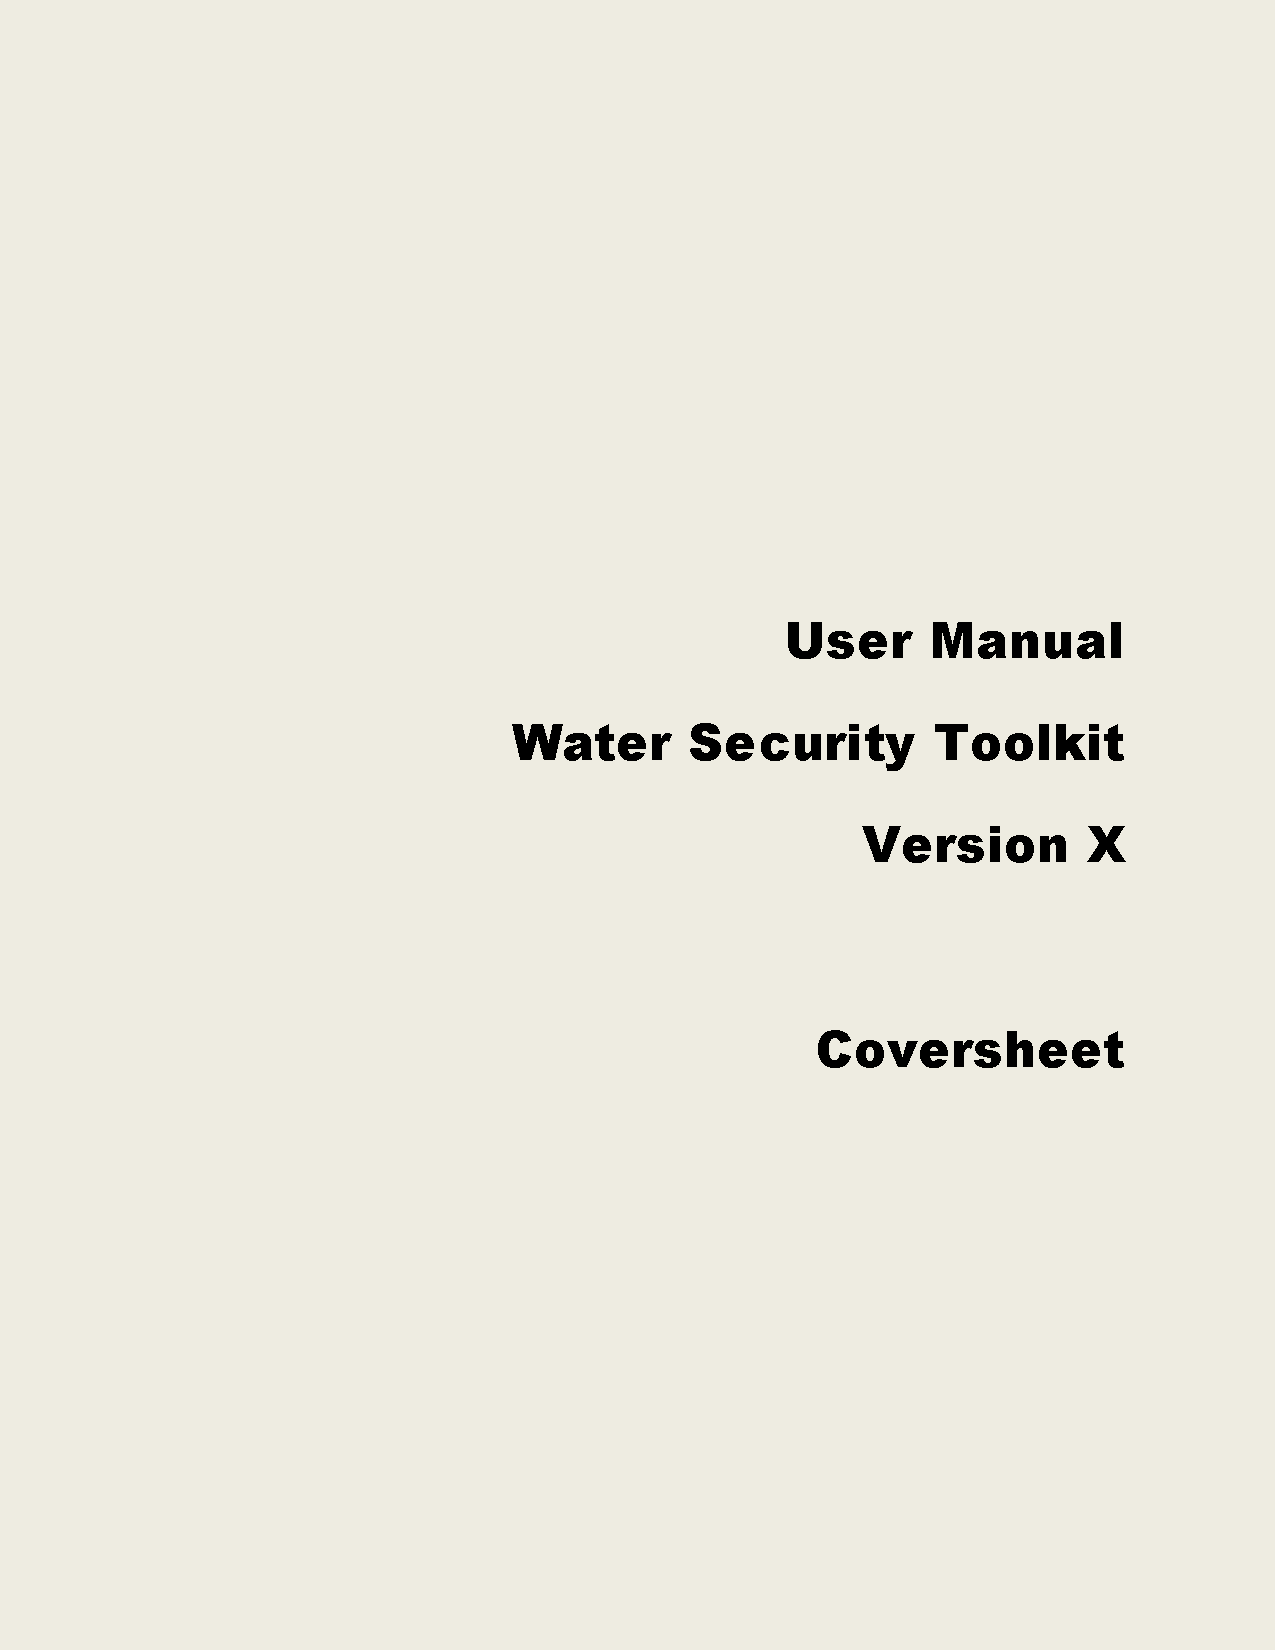
\includepdf[pages={1}]{last_page_blank.pdf}

  %% ==================================================================
  % END MAIN DOCUMENT
  %% ==================================================================
  
\end{document}

